\documentclass[
	aspectratio=169, % default is 43
	8pt, % font size, default is 11pt
	%handout, % handout mode without animations, comment out to add animations
]{beamer}
\def\university{magdeburg}

\documentclass[
	aspectratio=169, % default is 43
	8pt, % font size, default is 11pt
	handout, % handout mode without animations, comment out to add animations
]{beamer}

\usepackage{../template/beamerthemeuulm} % use the inofficial uulm beamer theme
\setfaculty{infIngPsy} % set the color scheme for your faculty here [med/infIngPsy/math/nat]

% requires symbolic links
% git clone git@github.com:SoftVarE-Group/SlideTemplate.git C:\Users\...\SlideTemplate
% mklink /J template C:\Users\...\SlideTemplate
% git clone git@spgit.informatik.uni-ulm.de:thuem/slides.git C:\Users\...\ThomasSlides
% mklink /J thomasslides C:\Users\...\ThomasSlides
\graphicspath{{../template/pics/logos}{../template/pics/nature}{../template/pics/uulm}{../thomasslides/}{../pics/people/}{../pics/xkcd/}}

%\usepackage[ngerman]{babel} % use this line for slides in German
%\recordingtrue % special recording mode for use with a greenscreen, gives you space to show yourself in a layer in front of the slides, has no effect in the handout mode

\title{Software Product Lines} % short title is used for the slide footer but optional

% LINKED LITERATURE

\newcommand{\ludewiglichter}{\href{https://learning.oreilly.com/library/view/-/9781457184932/?ar}{Ludewig and Lichter}}
\newcommand{\seeconomics}{\href{https://rds-ulm.ibs-bw.de/link?kid=027381854}{SE Economics}}
\newcommand{\sommervillelink}[1]{\href{https://ulm.ibs-bw.de/aDISWeb/app?service=direct/0/Home/$DirectLink\&sp=SOPAC00\&sp=SAKSWB-IdNr1615420983}{#1}}
\newcommand{\sommerville}{\sommervillelink{Sommerville}}
\newcommand{\thehumbleprogrammer}{\href{https://dl.acm.org/doi/10.1145/1283920.1283927}{The Humble Programmer}}
\newcommand{\thepragmaticprogrammer}{\href{https://learning.oreilly.com/library/view/the-pragmatic-programmer/9780135956977/}{The Pragmatic Programmer}}

% TYPICAL COMMANDS FOR LECTURES

\renewcommand{\emph}[1]{{\color{blue}\textbf{#1}}}

\newcommand{\deutsch}[1]{{\color{blue}(#1)}}
\newcommand{\deutschertitel}[1]{{\tiny\deutsch{#1}}}

\newcommand{\mycite}[1]{``#1''}
\newcommand{\mytitlesource}[1]{{\tiny\normalfont\mbox{[#1]}}}
\newcommand{\mysource}[1]{\ifthenelse{\equal{#1}{}}{}{\phantom{.}~\hfill~\mytitlesource{#1}}}

\newcommand{\todo}[1]{{\color{red}\textbf{[#1]}}}
\newcommand{\fodo}[1]{\todo{\footnote{\todo{#1}}}}
\newcommand{\todots}{\todo{\ldots}}

% IMPORTED PACKAGES

%\usepackage{adjustbox} % used for partofpage
%\usepackage{tcolorbox} % used for mydefinition, mynote, myexample
\usepackage{multicol} % used temporarily for the lecture overview
\usepackage{mathtools} % required for absolute value in modeling lecture

% COMMANDS TO LAYOUT AND ANNIMATE SLIDES

\newcommand{\lessonslearned}[3]{
	\subsection{Summary}
	\begin{frame}{\insertsection -- \insertsubsection}
		\leftorright{
			\mydefinition{Lessons Learned}{
				\begin{itemize}
					#1
				\end{itemize}
			}
			\mynote{Further Reading}{
				\small % references take space, can be a little smaller
				\begin{itemize}
					#2
				\end{itemize}
			}
		}{
			\myexample{Practice}{
				#3
			}
		}
	\end{frame}
}

% TODO temporary hack to layout the slide overview in two colums
\renewcommand{\lectureoverview}{
%	\section*{Overview}
%	\subsection*{Overview}
	\begin{frame}{\insertsubtitle}
		\begin{multicols}{2}
			\tableofcontents
		\end{multicols}
	\end{frame}
}

\renewcommandx{\maketitle}[2][1=apr21-o25a,2=150]{
    {
	\usebackgroundtemplate{} % TODO temporary hack to enable missing pictures at title slide
	%\ifx {#1} \empty \else {\usebackgroundtemplate{\includegraphics[trim=0 0 0 #2,clip,width=\paperwidth]{#1}}} \fi     
	%\usebackgroundtemplate{\includegraphics[trim=0 0 0 #2,clip,width=\paperwidth]{#1}}
    \begin{frame}[plain]
        \vskip0pt plus 1filll
        \begin{beamercolorbox}[wd=\paperwidth,ht=4.5ex,dp=2ex,right]{titlebox}
            \LARGE\textbf{\inserttitle}\hspace*{20pt}
        \end{beamercolorbox}%
        \nointerlineskip%
        \begin{beamercolorbox}[wd=\paperwidth,ht=2.25ex,dp=1ex,right]{subtitlebox}
            \small 
            \ifx \insertsubtitle \empty \else \insertsubtitle\ $\vert$ \fi
            \insertauthor\
            \ifx \insertdate \empty \else $\vert$ \insertdate \fi
            \hspace*{20pt}
        \end{beamercolorbox}%
        \nointerlineskip%
        \begin{beamercolorbox}[wd=\paperwidth,ht=4.5ex,dp=2ex,left]{logobox}
            \centering
            \vspace{-1ex}
            \hspace{10pt}
            \includegraphics[height=4.5ex]{sp} % SPECIFY INSTITUTE LOGO HERE
            \hfill
            \includegraphics[height=4.5ex]{uulm}
            \hspace{10pt}
        \end{beamercolorbox}%
    \end{frame}
    }  
}

%
%\newcommand{\onlyleft}[1]{
%	\halfpage{#1}
%}
%
%\newcommand{\onlyright}[1]{
%	~\hfill
%	\halfpage{#1}
%}
%
%\newcommand{\leftorright}[2]{
%	\uncover<1>{\halfpage{#1}}
%	\hfill
%	\uncover<3->{\halfpage{#2}}
%}
%
%\newcommand{\rightorleft}[2]{
%	\uncover<3->{\halfpage{#1}}
%	\hfill
%	\uncover<1>{\halfpage{#2}}
%}
%
%\newcommand{\leftthenright}[2]{
%	\halfpage{#1}
%	\hfill\pause
%	\halfpage{#2}
%}
%
%\newcommand{\leftandright}[2]{
%	\halfpage{#1}
%	\hfill
%	\halfpage{#2}
%}
%
%\newcommand{\leftmiddleandright}[3]{
%	\thirdpage{#1}
%	\hfill
%	\thirdpage{#2}
%	\hfill
%	\thirdpage{#3}
%}
%
%\newcommand{\leftmiddleorright}[3]{
%	\uncover<1>{\thirdpage{#1}}
%	\hfill
%	\uncover<3>{\thirdpage{#2}}
%	\hfill
%	\uncover<5->{\thirdpage{#3}}
%}
%
%\newcommand{\halfpage}[1]{\partofpage{48}{#1}}
%
%\newcommand{\thirdpage}[1]{\partofpage{31}{#1}}
%
%\newcommand{\partofpage}[2]{
%	\adjustbox{valign=t}{\begin{minipage}{0.#1\textwidth}
%			\begin{flushleft}
%				#2
%			\end{flushleft}
%	\end{minipage}}
%}
%
%\newcommand{\mydefinition}[2]{
%	\begin{tcolorbox}[title=#1,colback=orange!10,colframe=orange!30,coltitle=black,fonttitle=\bfseries,left=1mm,right=1mm,top=1mm,bottom=1mm]
%		\begin{flushleft}
%			#2
%		\end{flushleft}
%	\end{tcolorbox}
%}
%
%\newcommand{\mydefinitiontight}[2]{
%	\begin{tcolorbox}[title=#1,colback=white,colframe=orange!30,coltitle=black,fonttitle=\bfseries,left=0mm,right=0mm,top=0mm,bottom=0mm]
%		\begin{flushleft}
%			#2
%		\end{flushleft}
%	\end{tcolorbox}
%}
%
%\newcommand{\mynote}[2]{
%	\begin{tcolorbox}[title=#1,colback=red!10,colframe=red!30,coltitle=black,fonttitle=\bfseries,left=1mm,right=1mm,top=1mm,bottom=1mm]
%		\begin{flushleft}
%			#2
%		\end{flushleft}
%	\end{tcolorbox}
%}
%
%\newcommand{\myexample}[2]{
%	\begin{tcolorbox}[title=#1,colback=blue!10,colframe=blue!30,coltitle=black,fonttitle=\bfseries,left=1mm,right=1mm,top=1mm,bottom=1mm]
%		\begin{flushleft}
%			#2
%		\end{flushleft}
%	\end{tcolorbox}
%}
%
%\newcommand{\myexampletight}[2]{
%	\begin{tcolorbox}[title=#1,colback=white,colframe=blue!30,coltitle=black,fonttitle=\bfseries,left=0mm,right=0mm,top=0mm,bottom=0mm]
%		\begin{flushleft}
%			#2
%		\end{flushleft}
%	\end{tcolorbox}
%}

\subtitle{9. Feature Interactions}
\author{Thomas Thüm, Timo Kehrer, Elias Kuiter}
\foruniversity{}
	{\setpicture[35]{ovgu-winter3}\setcopyright{Photo: Hannah Theile (OVGU)}}
	{\setpicture{oct20-south4}}

\begin{document}

\mode<handout>{\contentoverview}

\mode<beamer>{
	\ifdefined\thepicture
		\maketitle[\thepicture][\thepictureoffset]
	\else
		\maketitle[]
	\fi
}

% shared slide content

% introduced: 02a-configuration
% reused: 03a-intro
\newcommand{\frameImplementSPLs}{
	\begin{mycolumns}[widths={45},animation=none]
		\pic[width=\linewidth]{metaproduct2}
	\mynextcolumn
		\begin{note}{Key Issues}
			\begin{itemize}
			\item Systematic reuse of implementation artifacts
			\item Explicit handling of variability
			\end{itemize}
		\end{note}
		\uncover<2->{\begin{definition}{Variability\mysource{\fospl\mypage{48}}}
			\mycite{\emph{Variability} is the ability to derive different products from a common set of artifacts.}
		\end{definition}}
		~
		\uncover<3->{\begin{note}{Variability-Intensive System}
			Any software product line is a variability-intensive system. % TODO Timo: do we really need this term? where does this definition come from?
		\end{note}}
	\end{mycolumns}
}

% introduced: 02a-configuration
% reused: 02b-implementation, 03a-intro
\newcommand{\frameVariabilityAndBindingTimes}{
	\begin{mycolumns}[widths={55},animation=none]
		\begin{definition}{Binding Time \deutsch{Bindungszeitpunkt}\mysource{\fospl\mypage{48}}}
			\begin{itemize}
				\item Variability offers choices
				\item Derivation of a product requires to make decisions (aka. binding)
				\item Decisions may be bound at different binding times
			\end{itemize}
		\end{definition}
		~
		\uncover<2->{\begin{note}{When? By whom? How?}
			\lectureruntime\parta: \emph{when} and \emph{by whom}

			\lectureruntime\partb: \emph{how}
		\end{note}}
	\mynextcolumn
		\pic[width=\linewidth]{metaproduct2}
	\end{mycolumns}
}

% introduced: 03a-intro
% reused: 03a-intro
\newcommand{\frameRuntimeVariabilityProblems}{
	\begin{note}{Problems of Runtime Variability}
		{\bf Conditional Statements:}
		\begin{itemize}
			\item Code scattering, tangling, and replication
		\end{itemize}
		{\bf Design Patterns for Variability:}
		\begin{itemize}
			\item Trade-offs and potential negative side effects
			\item Constraints that may restrict their usage
		\end{itemize}
		{\bf In General:}
		\begin{itemize}
			\item Variable parts are always delivered
			\item Not well-suited for compile-time binding
		\end{itemize}
	\end{note}
}

% introduced: 03a-intro
% reused: 03a-intro
\newcommand{\frameSoftwareConfigurationManagement}{
	\begin{mycolumns}
		\begin{definition}{Software Configuration Management} % TODO source missing
			Policies, processes, and tools for managing evolving software systems:
			\begin{itemize}
				\item Version control
				\item System building
				\item Release management
				\item Change management
				\item Collaborative work
			\end{itemize}
		\end{definition}
	\mynextcolumn
		\begin{note}{No Software Configuration Management}
			\lecturecloneandown\parta: Ad-Hoc Clone-and-Own

			aka.\ unmanaged clone-and-own
		\end{note}
		\begin{note}{Version Control}
			\lecturecloneandown\partb: Clone-and-Own with Version Control

			instance of managed clone-and-own
		\end{note}
		\begin{note}{System Building}
			\lecturecloneandown\partc: Clone-and-Own with Build Systems

			instance of managed clone-and-own
		\end{note}
	\end{mycolumns}
}


\begin{frame}{\inserttitle}
	\lectureseriesoverview[III]
\end{frame}

% TODO move to Lecture 10?
%\subsection{Recap: Software Quality}
%\begin{frame}{\myframetitle} % caution: slide copied from testing lecture
%	\rightorleft{
%		\mydefinition{Quality \mysource{\ludewiglichter}}{Quality is the entirety of properties and characteristics of a product or process that indicate adequacy with respect to given requirements.}
%		\mydefinition{Quality Assurance \mysource{\ludewiglichter}}{Quality assurance \deutsch{Qualitätssicherung} are all activities with the goal to improve the quality.}
%	}{
%		\vspace{-12mm}
%		\centering
%		\pic[width=\linewidth,trim=0 240 0 300,clip]{andy-hunt}
%		\vspace{-7mm}
%		
%		\mynote{Andy Hunt \mysource{\thepragmaticprogrammer}}{\mycite{No one in the brief history of computing has ever written a piece of perfect software. It's unlikely that you'll be the first.}}
%		% co-authored The Pragmatic Programmer, known for the Agile Manifesto
%	}
%\end{frame}

\section{What is a Feature Interaction?}

\subsection{Examples for Feature Interactions}

% TODO more ideas for examples
% beamer+notebook
% esp+abs: both control brakes and motor

\begin{frame}{An Interaction when Customizing Clothes}
	\begin{fancycolumns}[widths={33},animation=none]
		\begin{example}{Customization of Clothes}
			\begin{itemize}
			\item platforms to create and buy clothes
			\item creator preselects clothes with certain colors
			\item customization with pictures in different colors
			\item where is the problem?
			\end{itemize}
		\end{example}
	\nextcolumn
		\mywhite{uulm Shop \mysource{\href{https://uulm.myspreadshop.de/collections}{myspreadshop.de}}}{
			\pic[height=40mm]{spreadshirt-shop-2}
			\hfill
			\pic[height=40mm]{spreadshirt-shop-3}
		} % TODO exampletight with white background in darkmode
	\end{fancycolumns}
\end{frame}
\begin{frame}{An Interaction when Customizing Clothes}
	\begin{fancycolumns}
		\begin{exampletight}{The Problem: Unwanted Interaction of Colors}
			~

			\centering\picDark[height=50mm]{spreadshirt-email-1}

			~
		\end{exampletight}
	\nextcolumn
		\begin{exampletight}{The Solution: Choose Other Colors}
			~

			\centering\picDark[height=50mm]{spreadshirt-email-4}

			~
		\end{exampletight}
	\end{fancycolumns}
\end{frame}
\begin{frame}{An Interaction when Customizing Clothes}
	\begin{fancycolumns}
		\mywhite{The Problem: Unwanted Interaction of Colors}{
			\centering\pic[height=45mm,trim=50 3550 690 3340,clip]{spreadshirt-order}
		} % TODO exampletight with white background in darkmode
	\nextcolumn
		\mywhite{The Solution: Choose Other Colors}{
			\centering\pic[height=45mm,trim=50 3255 690 3635,clip]{spreadshirt-order}
		} % TODO exampletight with white background in darkmode
	\end{fancycolumns}
	\uncover<3->{\begin{note}{}
		\centering seems that contrast is checked for each order (cf.\ application engineering)\\and not for each published design (cf.\ domain engineering)
	\end{note}}
\end{frame}
% TODO add links to keynote?

\begin{frame}{An Interaction of Android Apps}
	\begin{fancycolumns}[widths={67},animation=none]
		\mywhite{}{\only<1-2|handout:0>{\pic[width=\linewidth,page=11,trim=40 30 280 100,clip]{2021/2021-09-08-SPLC-Keynote}}%
		\only<3->{\pic[width=\linewidth,page=11,trim=40 30 40 100,clip]{2021/2021-09-08-SPLC-Keynote}}}%
		\only<4->{\begin{note}{}%
			\centering which of those 3.5 million Android apps interact?\\where to document?\\whom to blame?%
		\end{note}}%
	\nextcolumn
		\begin{example}{Skype vs BabyMonitor}
			\begin{itemize}
			\item Skype app installed and used for years
			\item BabyMonitor installed, carefully tried and used for months
			\item BabyMonitor can call any other number (i.e., works without internet)
			\item automatic update of the Skype app
			\item update causes a question to be asked for every call
			\item \alt<-2>{what is the problem?}{found baby crying as no one answered the dialog}
			\end{itemize}
		\end{example}
	\end{fancycolumns}
\end{frame}
% TODO use pictures directly, add picture showing all apps
% TODO add links to keynote?

%\begin{frame}{Can We Trust Our Scans?}
%	\centering\pic[width=\linewidth,page=28,trim=40 30 40 70,clip]{2021/2021-09-08-SPLC-Keynote}
%\end{frame}
% TODO add scanner example? is it really dependent on multiple options? or only on one particular setting

\subsection{Feature Interactions}
\begin{frame}{\myframetitle}
	\begin{fancycolumns}
		\begin{definition}{Feature Interaction\mysource{\fospl\mypage{214}}}
			\mycite{A \emph{feature interaction} between two or more features is an
emergent behavior that cannot be easily deduced from the behaviors associated
with the individual features involved.}

			for short: interaction
		\end{definition}
		\begin{definition}{Inadvertent Interaction\mysource{\fospl\mypage{214}}}
			\mycite{An \emph{inadvertent feature interaction} occurs when a feature influences the behavior of another feature in an unexpected way (for example, regarding the expected control flow, program or data state, or visible behavior).}

			here simplified as: wanted vs unwanted
		\end{definition}
	\nextcolumn
		\begin{definition}{Feature-Interaction Problem\mysource{\fospl\mypage{214}}}
			\mycite{The \emph{feature-interaction problem} is to detect, manage, and resolve (inadvertent) feature interactions among features.}
		\end{definition}
		\begin{note}{Feature Interactions}
			\begin{itemize}
				\item detection discussed in next two lectures \mysource{\lectureanalyses\ and \lecturetesting}
				\item resolving interactions (see Part II)
				\item managing interactions (see Part III)
			\end{itemize}
		\end{note}
		\begin{note}{What's Next?}
			\begin{itemize}
				\item interactions due to the absence of features
				\item interactions in source code
				\item interactions with the base code
			\end{itemize}
		\end{note}
	\end{fancycolumns}
\end{frame}

\begin{frame}{A Common Interaction of Toasters}
	\begin{fancycolumns}[animation=none]
		\only<1|handout:0>{\pic[width=\linewidth]{toast1}}%
		\only<2|handout:0>{\pic[width=\linewidth]{toast2}}%
		\only<3-|handout:1>{\pic[width=\linewidth]{toast3}}%
		\uncover<5->{\begin{example}{}
			\centering no interaction for two toasts (i.e., \emph{$T_1 \pand T_2$} shown) and for no toasts (i.e., $\pnot T_1 \pand \pnot T_2$ not shown)
		\end{example}}
	\nextcolumn
		\only<4->{\pic[width=\linewidth]{toast4}}%
		\uncover<6->{\begin{example}{}
			\centering unwanted interaction for one toast\\(i.e., \emph{$T_1 \pand \pnot T_2$} shown and  $\pnot T_1 \pand T_2$ not shown)
		\end{example}}
	\end{fancycolumns}
\end{frame}

\subsection{Example Interactions with Preprocessors}
\begin{frame}{\myframetitle}
	\begin{fancycolumns}[widths={70}]
		\only<1|handout:0>{\pic[width=\linewidth,page=1,trim=20 20 20 40,clip]{preprocessor-wilderness}}%
		\only<2->{\pic[width=\linewidth,page=2,trim=20 20 20 40,clip]{preprocessor-wilderness}}%
	\nextcolumn
		\begin{example}{No Interaction?}\setlength\leftmargini{3mm}
			\begin{itemize}
				\item configuration for undirected, weighted edges
				\item product can be compiled
				\item what is the problem?
			\end{itemize}
		\end{example}
	\end{fancycolumns}
\end{frame}
\begin{frame}{\myframetitle}
	\begin{fancycolumns}[widths={70}]
		\pic[width=\linewidth,page=4,trim=20 20 20 40,clip]{preprocessor-wilderness}
	\nextcolumn
		\begin{example}{Static Interaction}\setlength\leftmargini{3mm}
			\begin{itemize}
				\item configuration for undirected, unweighted edges
				\item product cannot be compiled due to static feature interaction
				\item field \emph{weight} used for undirected edges but defined in feature \emph{Weighted}
				\item occurs whenever features \emph{Directed} and \emph{Weighted} are both not selected
			\end{itemize}
		\end{example}
	\end{fancycolumns}
\end{frame}
\begin{frame}{\myframetitle}
	\begin{fancycolumns}[widths={70}]
		\pic[width=\linewidth,page=3,trim=20 20 20 40,clip]{preprocessor-wilderness}
	\nextcolumn
		\begin{example}{Other Static Interaction}\setlength\leftmargini{3mm}
			\begin{itemize}
				\item configuration for directed, weighted edges
				\item product cannot be compiled due to static feature interaction
				\item semicolon and bracket missing for every configuration with feature \emph{Directed}
				\item feature \emph{Directed} has inadvertent interaction with base code
			\end{itemize}
		\end{example}
	\end{fancycolumns}
\end{frame}
\begin{frame}{\myframetitle}\setlength\leftmargini{3mm}
	\begin{fancycolumns}[widths={70}]
		\pic[width=\linewidth,page=5,trim=20 20 20 40,clip]{preprocessor-wilderness}
	\nextcolumn
		\begin{example}{Dynamic Interaction?}
			\begin{itemize}
				\item again: configuration for undirected, weighted edges
				\item product can be compiled but test fails
				\item not a static interaction
				\item defect in the base code
				\item no interaction at all
			\end{itemize}
		\end{example}
		\begin{note}{Detection of Interactions}
			\begin{itemize}
				\item static interactions\\\mysource{\lectureanalyses}
				\item dynamic interactions\\\mysource{\lecturetesting}
				\item next: interactions of more than two features
			\end{itemize}
		\end{note}
	\end{fancycolumns}
\end{frame}

%\subsection{Unwanted and Wanted Interactions} % Desired + Undesired
% \href{https://github.com/SoftVarE-Group/Slides/blob/main/2021/2021-09-08-SPLC-Keynote.pdf}{\mycite{Every unwanted feature interaction waits to be fixed or at least documented in form of a constraint.}} T:SPLC21 

%\subsection{Pairwise Interactions}
\subsection{Higher-Order Interactions}
\begin{frame}{\myframetitle}
	\begin{fancycolumns}
		\begin{definition}{Kinds of Interactions}
			\begin{itemize}
				\item wanted and unwanted interactions
				\item static and dynamic interactions
				\item one-wise interactions (interaction of features with the base code and faulty features)
				\item pair-wise interactions (between two features)
				\item higher-order interactions (between more than two features)
			\end{itemize}
		\end{definition}
		\uncover<2->{\begin{example}{Variability Bug Database\mysource{\VBDb}}
			\begin{itemize}
				\item database of known feature interactions
				\item operating system Linux (43 interactions)
				\item web server Apache (23)
				\item system tool Busybox (18)
				\item 3D printer firmware Marlin (14)
			\end{itemize}
		\end{example}}
	\nextcolumn
		\begin{exampletight}{Patterns of Feature Interactions\mysource{\VBDb}}
			\pic[width=\linewidth]{variabilitybugdatabase-patterns}
		\end{exampletight}
	\end{fancycolumns}
\end{frame}
% TODO example from the The Variability Bug Database?

\begin{frame}{Interaction on Data and Control Flow \mytitlesource{\essentialconfigurationcomplexity}}\setlength\leftmargini{3mm}
	\begin{fancycolumns}[widths={70}]
		\mywhite{}{\essentialconfigurationcomplexitylink{\pic[width=\linewidth,page=2,trim=55 495 225 75,clip]{2016/2016-ASE-Meinicke}}}
	\nextcolumn
		\begin{note}{How do Features Interact?}
			\begin{itemize}
				\item given a program with runtime variability
				\item given one test case (i.e., concrete inputs)
				\item how much does the execution depend on the configuration?
				\item how many values for each variable? (green)
				\item how many different control flows? (red)
				\item blue color not relevant here (minimal overhead during simultaneous execution)
			\end{itemize}
		\end{note}
	\end{fancycolumns}	
\end{frame}
\begin{frame}[label=ExecutionTracesInConfigurableSystems]{Execution Traces in Configurable Systems \mytitlesource{\essentialconfigurationcomplexity}}
	\mywhite{}{\essentialconfigurationcomplexitylink{\pic[width=.95\linewidth,page=8,trim=55 520 55 55,clip]{2016/2016-ASE-Meinicke}}}

	\begin{note}{}
		\centering insights: not all features interact. some statements may lead to higher interactions than others.
	\end{note}
\end{frame}

% TODO explain duality between partial configurations and conjunctions of literals (cf. elevator product line by Varshosaz et al.)


\lessonslearned{
	\item feature interaction and feature-interaction problem
	\item wanted/unwanted, static/dynamic, one-wise/pair-wise/higher-order
	\item examples: customization of clothes, Android apps, toaster, preprocessor code, runtime variability, Variability Bug Database
}{
	\item \fospl\ Chapter 9 \mypages{213--217}
}{
	Do you know further examples of feature interactions?
}

\sectionend

\section{How to Handle Feature Interactions?}

%% discuss techniques and refer to previous examples (message: it depends when what is feasible)
%\subsection{S1: Exclude Feature Combinations}
%% example: leonovo option compatibility matrix (even if not strictly enforced)
%% example: web configurators (Thinkpad)
%\subsection{S2: Orthogonal Implementation}
%\subsection{S3: Duplicate Implementations}
%\subsection{S4: Move Source Code}
%\subsection{S5: Preprocessors}
%\subsection{S6: Derivative Modules}
%\subsection{Overview on all Strategies}
%\subsection{When to Handle?}
%% spreadshirt example: fixing foreground+background colors for every order


\subsection{Motivation}

\begin{frame}{Handling/Implementing Feature Interactions}
	\begin{mycolumns}[widths={50,50},animation=none]
		\mynote{Assumptions}{
			\begin{itemize}
				\item Interacting features have been already identified
				\item Interaction is a pairwise interaction (i.e., two features)
			\end{itemize}
		}
	\mynextcolumn
		\mydefinition{Problem Description}{
			\begin{itemize}
				\item Find a strategy to handle the interaction 
				\item Strategy does not introduce the optional-feature problem
			\end{itemize}
		}
	\end{mycolumns}
\end{frame}

\begin{frame}[fragile]{Example: A Feature Interaction in our Graph Library}
	\begin{mycolumns}[widths={50,50},animation=none]
		\myexampletight{}{
			\centering
			\featureDiagram{
				Graph,concrete
				[Nodes,mandatory,abstract
					[Colored,optional,concrete]]
				[Edges,mandatory,abstract
					[Directed,optional,concrete]
					[Weighted,optional,concrete]]
				[Algorithms,mandatory,abstract,
					[ShortestPath,optional,concrete]]
			}
		}
		\vspace{3mm}
		\mynote{}{
			\begin{itemize}
				\item Domain view: $Weighted$ and $ShortestPath$ can be deliberately selected independent of each other.
				\item Implementation view: $ShortestPath$ requires $Weighted$ due to an implementation dependency (optional-feature problem!).
			\end{itemize}
		}
	\mynextcolumn
{\small
\begin{codetight}{layer: BasicGraph}
class Edge {
	private Node a, b;
	...
}
\end{codetight}	
\begin{codetight}{layer: Weighted}
refines class Edge {
	double weight;
	void setWeight(double w){ ... }
}
\end{codetight}	
\begin{codetight}{layer: ShortestPath}
refines class Graph {
	List shortestPath(Node a, Node b){
		Edge e1, e2;
		...
		if(e1.weight > e2.weight) 
		... 
	}
}
\end{codetight}	
}
	\end{mycolumns}
\end{frame}

\begin{frame}{Handling/Implementing Feature Interactions: General Goals}
	\mynote{Question}{
		What makes a good strategy to implement coordination code for feature interactions (while solving/avoiding the optional-feature problem)?
	}
	\pause
	\begin{mycolumns}[widths={50,50},animation=none]
		\mydefinition{1. Variability}{
			For every valid configuration (according to feature model), we can generate a product that implements this configuration.
		}
		\pause
		\mydefinition{2. Implementation effort}{
			Should not require overwhelming implementation effort (would not be attractive in practice).
		}
		\pause
	\mynextcolumn
		\mydefinition{3. Binary size and performance}{
			Should not increase binary size or decrease performance of products compared to an individual implementation of each product.
		}
		\pause
		\mydefinition{4. Code quality}{
			Should not reduce code quality, which would make the product line harder to maintain. 
		}
	\end{mycolumns}
\end{frame}

\subsection{S1: Adapt Feature Model}

\begin{frame}{S1 (a): Adapt Feature Model - Add Domain Dependency}
	\mydefinition{Strategy}{
		Declare implementation dependency as domain dependency in the feature model.
	}
	\mynotetight{}{
		\centering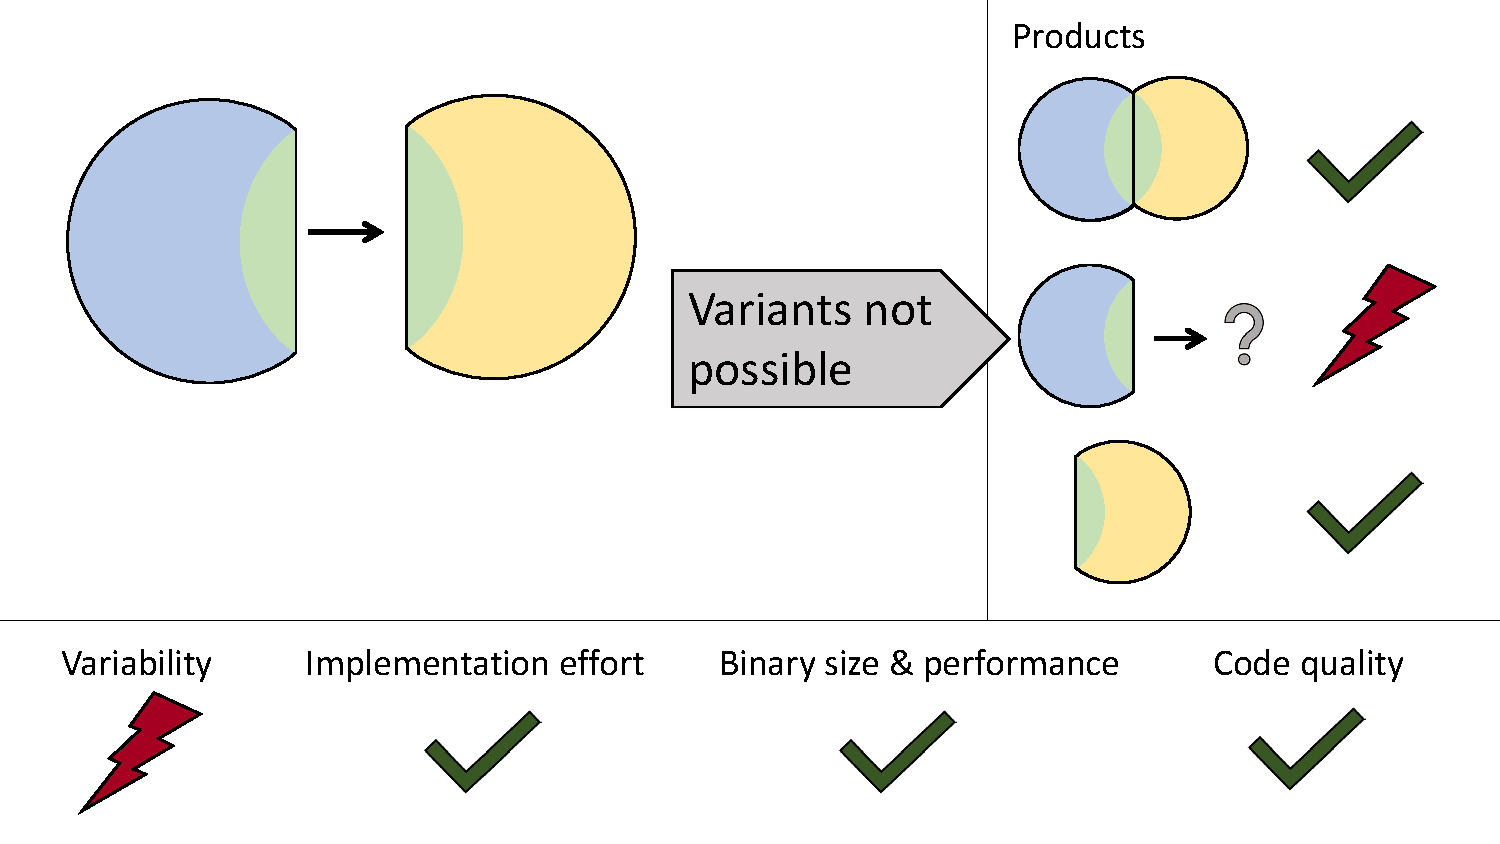
\includegraphics[width=0.7\linewidth,page=1]{interaction-handling}
	}
\end{frame}

\begin{frame}[fragile]{Example}
	\begin{mycolumns}[widths={50,50},animation=none]
		\myexampletight{}{
			\centering
			\featureDiagram{
				Graph,concrete
				[Nodes,mandatory,abstract
					[Colored,optional,concrete]]
				[Edges,mandatory,abstract
					[Directed,optional,concrete]
					[Weighted,optional,concrete]]
				[Algorithms,mandatory,abstract,
					[ShortestPath,optional,concrete]]
			}

			$ShortestPath \pimplies Weighted$  
		}
		\vspace{3mm}
		\mynote{}{
			Same implementation as before, but we make implementation dependency explicit: $ShortestPath$ requires $Weighted$.
		}
	\mynextcolumn
{\small
\begin{codetight}{layer: BasicGraph}
class Edge {
	private Node a, b;
	...
}
\end{codetight}	
\begin{codetight}{layer: Weighted}
refines class Edge {
	double weight;
	void setWeight(double w){ ... }
}
\end{codetight}	
\begin{codetight}{layer: ShortestPath}
refines class Graph {
	List shortestPath(Node a, Node b){
		Edge e1, e2;
		...
		if(e1.weight > e2.weight) 
		... 
	}
}
\end{codetight}	
}
	\end{mycolumns}
\end{frame}

\begin{frame}{S1 (b): Adapt Feature Model - Exclude Feature Combinations}
	\mydefinition{Strategy}{
		Declare problematic feature combinations as mutually exclusive in the feature model.
	}
	\mynotetight{}{
		\centering\includegraphics[width=0.7\linewidth,page=2]{interaction-handling}
	}
\end{frame}

\begin{frame}[fragile]{Example}
	\begin{mycolumns}[widths={50,50},animation=none]
		\myexampletight{}{
			\centering
			\featureDiagram{
				Graph,concrete
				[Nodes,mandatory,abstract
					[Colored,optional,concrete]]
				[Edges,mandatory,abstract
					[Directed,optional,concrete]
					[Weighted,optional,concrete]]
				[Algorithms,mandatory,abstract,
					[ShortestPath,optional,concrete]]
			}

			$\pnot (ShortestPath \pand Weighted)$  
		}
		\vspace{3mm}
		\mynote{}{
			We may safely assume any uniform weight because $ShortestPath$ and $Weighted$ are mutually exclusive.
		}
	\mynextcolumn
\vspace{-3mm}
{\small
\begin{codetight}{layer: BasicGraph}
class Edge {
	private Node a, b;
	...
}
\end{codetight}	
\begin{codetight}{layer: Weighted}
refines class Edge {
	double weight;
	void setWeight(double w){ ... }
}
\end{codetight}	
\begin{codetight}{layer: ShortestPath}
refines class Graph {
	List shortestPath(Node a, Node b){
		@float w1 = 1.0;@
		@float w2 = 1.0;@
		...
		@if(w1 > w2)@
		... 
	}
}
\end{codetight}	
}
	\end{mycolumns}
\end{frame}

\subsection{S2: Orthogonal Implementation}

\begin{frame}{\myframetitle}
	\mydefinition{Strategy}{
		Orthogonal implementation with no dedicated coordination of interaction.
	}
	\mynotetight{}{
		\centering\includegraphics[width=0.7\linewidth,page=3]{interaction-handling}
	}
\end{frame}

\begin{frame}[fragile]{Example}
	\begin{mycolumns}[widths={50,50},animation=none]
		\myexampletight{}{
			\centering
			\featureDiagram{
				Graph,concrete
				[Nodes,mandatory,abstract
					[Colored,optional,concrete]]
				[Edges,mandatory,abstract
					[Directed,optional,concrete]
					[Weighted,optional,concrete]]
				[Algorithms,mandatory,abstract,
					[ShortestPath,optional,concrete]]
			}

			$\pnot (ShortestPath \pand Weighted)$  
		}
		\vspace{3mm}
		\mynote{}{
			Calculation of shortest path ignores weights but merely counts the number of edges on a path.
		}
	\mynextcolumn
{\small
\begin{codetight}{layer: BasicGraph}
class Edge {
	private Node a, b;
	...
}
\end{codetight}	
\begin{codetight}{layer: Weighted}
refines class Edge {
	double weight;
	void setWeight(double w){ ... }
}
\end{codetight}	
\begin{codetight}{layer: ShortestPath}
refines class Graph {
	List shortestPath(Node a, Node b){
		@// ignore weights@
		... 
	}
}
\end{codetight}	
}
	\end{mycolumns}
\end{frame}

\subsection{S3: Duplicate Implementations}

\begin{frame}{\myframetitle}
	\mydefinition{Strategy}{
		Multiple implementations of a feature, with and without coordination code.
	}
	\mynotetight{}{
		\centering\includegraphics[width=0.7\linewidth,page=4]{interaction-handling}
	}
\end{frame}

\begin{frame}[fragile]{Example}
	\begin{mycolumns}[widths={50,50},animation=none]
\begin{codetight}{layer: ShortestPath\_Unweighted}
refines class Graph {
	List shortestPath(Node a, Node b){
		...
		...
		// ignore weights
		... 
	}
}
\end{codetight}
		\mynote{}{			
			Selected iff $ShortestPath \pand \pnot Weighted$. 
		}
	\mynextcolumn
\begin{codetight}{layer: ShortestPath\_Weighted}
refines class Graph {
	List shortestPath(Node a, Node b){
		Edge e1, e2;
		...
		if(e1.weight > e2.weight) 
		... 
	}
}
\end{codetight}	
		\mynote{}{
			Selected iff $ShortestPath \pand Weighted$.
		}
	\end{mycolumns}
\end{frame}

\subsection{S4: Move Source Code}

\begin{frame}{\myframetitle}
	\mydefinition{Strategy}{
		Move all the coordination code to one of the features (or to a third one all interacting features depend on).
	}
	\mynotetight{}{
		\centering\includegraphics[width=0.7\linewidth,page=5]{interaction-handling}
	}
\end{frame}

\begin{frame}[fragile]{Example}
	\begin{mycolumns}[widths={50,50},animation=none]
\begin{codetight}{layer: BasicGraph}
class Edge {
	private Node a, b;
	@double weight = 1.0;@
	...
}
\end{codetight}	
\begin{codetight}{layer: Weighted}
refines class Edge {
	void setWeight(double w){ ... }
}
\end{codetight}	
	\mynextcolumn
\begin{codetight}{layer: ShortestPath}
refines class Graph {
	List shortestPath(Node a, Node b){
		Edge e1, e2;
		...
		if(e1.weight > e2.weight) 
		... 
	}
}
\end{codetight}	
	\end{mycolumns}
\end{frame}

\subsection{S5: Conditional Compilation}

\begin{frame}{\myframetitle}
	\mydefinition{Strategy}{
		Coordination code is only executed if both features are selected.
	}
	\mynotetight{}{
		\centering\includegraphics[width=0.7\linewidth,page=6]{interaction-handling}
	}
\end{frame}

\begin{frame}[fragile]{Example}
	\begin{mycolumns}[widths={50,50},animation=none]
\begin{codetight}{layer: BasicGraph}
class Edge {
	private Node a, b;
	...
}
\end{codetight}	
\begin{codetight}{layer: Weighted}
refines class Edge {
	double weight;
	void setWeight(double w){ ... }
}
\end{codetight}	
	\mynextcolumn
\begin{codetight}{layer: ShortestPath}
refines class Graph {
	List shortestPath(Node a, Node b){
		Edge e1, e2;
		...
@#ifdef WEIGHTED@		
		if(e1.weight > e2.weight) ...
@#endif@
		... 
	}
}
\end{codetight}	
	\end{mycolumns}
\end{frame}

\subsection{S6: Derivative Modules}

\begin{frame}{\myframetitle}
	\mydefinition{Strategy}{
		Create a dedicated module for code that coordinates features.
	}
	\mynotetight{}{
		\centering\includegraphics[width=0.7\linewidth,page=7]{interaction-handling}
	}
\end{frame}

\begin{frame}[fragile]{Example}
	\begin{mycolumns}[widths={50,50},animation=none]
\begin{codetight}{layer: ShortestPath}
refines class Graph {
	List shortestPath(Node a, Node b){
		Edge e1, e2;
		...
		if(isLonger(e1,e2)) 
		... 
	}
	boolean isLonger(Edge e1, Edge e2){
		return false;
	}
}
\end{codetight}	
	\mynextcolumn
\begin{codetight}{layer: ShortestPath\_Weighted}
refines class Graph {
	boolean isLonger(Edge e1, Edge e2){
		return e1.weight > e2.weight;
	}
}
\end{codetight}	
		\mynote{}{			
			Selected iff $ShortestPath \pand Weighted$. 
		}	
	\end{mycolumns}
\end{frame}

\subsection{Overview and Discussion}

\begin{frame}{Overview and Discussion}
	\centering\includegraphics[width=0.9\linewidth,page=8,trim=40 25 40 25,clip]{interaction-handling}
\end{frame}




\lessonslearned{
	\item Adaptation of feature model to avoid (undesired) feature interactions. 
	\item Strategies to implement coordination code for known feature interactions.
	\item Discussion of the strenghts and weaknesses of each of the strategies.
}{
	\item Kästner et al.: On the impact of the optional feature problem: Analysis and case studies. SPLC 2009.
	\item \fospl, Chapter 9
}{
	Looking back at our graph library and the feature interaction between $ShortestPath$ and $Weighted$. Which strategy would you choose to handle this interaction? Why?
	
	Can you think of other feature interactions for the graph library (you may also add additional features)? Again, how would you handle them? 
}

\sectionend

\section{How to Avoid Feature Interactions?}

% TODO \subsection{Recap: Size of Configuration Spaces}

% TODO \subsection{Recap: Increase of Features and Variants}
% features: Linux
% variants: Automotive02-05, KfW?

% TODO number of potential interactions?

% TODO variant reduction, prevent the explosion. marketing wants them all. engineering and quality assurance too expensive.

%\subsection{Domain Scoping Revisited}

%\subsection{Costs of Variability}

\subsection{The Choice of Features}
\begin{frame}{\myframetitle}
	\begin{mycolumns}
		\begin{exampletight}{John Ferguson Smart (2017)}
			\picDark[width=.98\linewidth,angle=2,trim=0 0 5 0,clip]{unnecessary-features}
		\end{exampletight}
		% 
	\mynextcolumn
		\centering\pic[width=.47\linewidth]{john-carmack}
		\vspace{-7mm}
		
		\begin{note}{John Carmack (born 1970) \mysource{\href{https://www.ics.uci.edu/~pattis/quotations.html\#C}{uci.edu}}}
			\mycite{The important point is that the cost of adding a feature isn't just the time it takes to code it. The cost also includes the addition of an obstacle to future expansion. %Sure, any given feature list can be implemented, given enough coding time. But in addition to coming out late, you will usually wind up with a codebase that is so fragile that new ideas that should be dead-simple wind up taking longer and longer to work into the tangled existing web. 
		[...] The trick is to pick the features that don't fight each other.}
		\end{note}
		% video game developer, co-founder of a video game company
	\end{mycolumns}
\end{frame}

\begin{frame}{\myframetitle}
	\begin{mycolumns}[animation=none]
		\pic[width=\linewidth]{ford-t-1910}
	\mynextcolumn
		\begin{note}{Henry Ford, 1909} % TODO source for this quote missing
			\mycite{Any customer can have a car painted any color that he wants so long as it is black.}
		\end{note}
		\uncover<2->{\begin{example}{Why only black?\mysource{\fospl}}
			\begin{itemize}
				\item black color dried faster
				\item faster production
				\item more products and cheaper production
			\end{itemize}
		\end{example}}
	\end{mycolumns}
\end{frame}

\subsection{Documentation of Interactions}

\subsubsection*{Incompatibilities of Lenovo Hardware}
\begin{frame}{\myframetitle}
	\begin{mycolumns}[widths={59}]
		\begin{note}{Documentation of Remaining Interactions}
			\begin{itemize}
				\item not all interactions can be prevented/fixed
				\item how to apply strategy S1 (see Part II) if there is no feature model?
				\item what to document?
			\end{itemize}
		\end{note}
		\uncover<2->{\begin{example}{Lenovo's Option Compatibility Matrices}
			\begin{itemize}
				\item 7 Excel files for current products\\+ archive for old products
				\item Excel file for computers contains 32 tables (series)
				\item table for ThinkPad X has 28 columns (models) and $>500$ rows (accessories)
				\item 14k cells contain $>400$ different footnotes
				\item a footnote explains one incompatibility
			\end{itemize}
		\end{example}}
	\mynextcolumn
		\myexampletight{}{
			\picDark[width=\linewidth,trim=0 1900 0 0,clip]{lenovo-compatibility-matrices}
			\picDark[width=\linewidth,trim=0 1130 0 600,clip]{lenovo-compatibility-matrices}
		}
	\end{mycolumns}
\end{frame}
\begin{frame}{\myframetitle}
	\begin{mycolumns}[widths={80},animation=none]
		\picDark[width=\linewidth]{lenovo-compatibility-matrix-1}
	\mynextcolumn
		\begin{example}{}\setlength\leftmargini{3mm} 
			\begin{itemize}
				\item columns contain notebooks
				\item rows contain accessories
				\item X indicates compatibility
				\item numbers indicate a known incompatibility
			\end{itemize}
		\end{example}
	\end{mycolumns}
\end{frame}
\begin{frame}{\myframetitle}
	\begin{mycolumns}[widths={80},animation=none]
		\picDark[width=\linewidth]{lenovo-compatibility-matrix-3}
	\mynextcolumn
		\begin{example}{}\setlength\leftmargini{3mm} 
			\begin{itemize}
				\item 314: pen requires touch screen (cf.\ S1)
				\item 315/319/320: extra module needed (cf.\ S6)
				\item 316/317: fixed in newer BIOS versions
				\item 318/321: two modules with a different power supply (cf.\ S3)
			\end{itemize}
		\end{example}
	\end{mycolumns}
\end{frame}


\lessonslearned{
	\item reduction of variability
	\item which features are actually needed?
	\item documentation of interactions that cannot be avoided
}{
	\item[] 
}{
	Who checks the compatibility of Lenovo products?
}

\mode<beamer>{
	\begin{frame}{\inserttitle}
		\lectureseriesoverview
	\end{frame}

	\contentoverview
}


\end{document}
